\documentclass{article}

\title{Dummit \& Foote Ch. 3.3: The Isomorphism Theorems}
\author{Scott Donaldson}
\date{Oct. 2023}
\usepackage{amsmath, amsthm, amsfonts, amssymb, enumitem, tabu, tikz}

\begin{document}

\maketitle

Let $G$ be a group.

\section*{1. (10/20/23)}

Let $F$ be a finite field of order $q$ and let $n \in \mathbb{Z}^+$. Prove that \\ $|GL_n(F) : SL_n(F)| = q - 1$.

\begin{proof}
    Define a map $\varphi: GL_n(F) \rightarrow F^\times$ by $\varphi(A) = \det A$ for all $A \in GL_n(F)$. From Ch. 3.1, Exercise 35., $\varphi$ is a surjective homomorphism with $\ker \varphi = SL_n(F)$.

    From Corollary 17, we have:
    \begin{align*}
        |GL_n(F) : \ker \varphi| &= |\varphi(GL_n(F))|, \text{ which implies that} \\
        |GL_n(F) : SL_n(F)| &= \underbrace{|F^\times|}_\text{$\varphi$ is surjective} = q - 1,
    \end{align*}
    as desired.
\end{proof}

% \section*{2. (10/26/23)}

% Prove all parts of the Lattice Isomorphism Theorem.

% The Lattice Isomorphism Theorem states that, if $N \unlhd G$, then there is a bijection from the set of subgroups $A$ of $G$ which contain $N$ onto the set of subgroups $\overline{A} = A/N$ of $G/N$. This bijection has the following properties:
% \begin{enumerate}[itemsep=0em]
%     \item $A \leq B$ if and only if $\overline{A} \leq \overline{B}$:
%         \begin{proof}
%             If $A \leq B$, then $a \in A$ implies $a \in B$. It follows that $\overline{a} = aN \in B/N$, so $A/N \leq B/N$.

%             Conversely, if $A/N \leq B/N$ and we let $a \in A$, then $\overline{a} = aN \in B/N$ Therefore $a$ is a representative of a coset in $B/N$, so $a \in B$, and therefore $A \leq B$.
%         \end{proof}
%     \item If $A \leq B$, then $|B:A| = |\overline{B}:\overline{A}|$:
%         \begin{proof}
            
%         \end{proof}
% \end{enumerate}

\section*{3. (10/26/23)}

Prove that if $H$ is a normal subgroup of $G$ of prime index $p$ then for all $K \leq G$ either
\begin{enumerate}[label=(\roman*), itemsep=0em]
    \item $K \leq H$ or
    \item $G = HK$ and $|K : K \cap H| = p$. 
\end{enumerate}

\begin{proof}
    Suppose that $H \unlhd G$ with $|G:H| = |G/H| = p$, where $p$ is a prime. Suppose additionally that $K \leq G$ and $K \nleq H$.

    Now let $g \in G$. Clearly $g$ belongs to the left coset $gH$, which we denote $\overline{g} \in G/H$. Since $G/H$ has order $p$, it is cyclic, and so is generated by any non-identity element (that is, any coset of $H$ other than itself). So $\overline{g}$ generates $G/H$. Similarly, for any $k \in K, k \notin H$, $\overline{k}$ generates $G/H$. Therefore $\overline{g} = \overline{k}$ for some $g, k$, which implies that $g \in kH$. It follows that $g \in KH$, so $G \leq KH$. Since $G$ is closed, we must have $G = KH = HK$.

    From the Diamond Isomorphism Theorem, we have $HK / H \cong K / H \cap K$. Since $HK = G$, it follows that $|G : H| = |K : H \cap K|$, and so $|K : K \cap H| = p$.
\end{proof}

\section*{4. (10/27/23)}

Let $C$ be a normal subgroup of the group $A$ and let $D$ be a normal subgroup of the group $B$. Prove that $(C \times D) \unlhd (A \times B)$ and $(A \times B)/(C \times D) \cong (A / C) \times (B / D)$.

\begin{proof}
    Let $(c, d) \in C \times D$. Consider the conjugate of $(c, d)$ by $(a, b) \in A \times B$:
    \begin{equation*}
        (a, b)(c, d)(a, b)^{-1} = (a, b)(c, d)(a^{-1}, b^{-1}) = (aca^{-1}, bdb^{-1}).
    \end{equation*}
    Because $C \unlhd A$, the first coordinate is an element of $C$, and similarly the second is an element of $D$. Therefore the conjugate element lies in $C \times D$, and it follows that $(C \times D) \unlhd (A \times B)$.

    Next, to show that $(A \times B)/(C \times D) \cong (A / C) \times (B / D)$, define a map $\varphi: (A \times B)/(C \times D) \rightarrow (A / C) \times (B / D)$ by $\varphi((\overline{a, b})) = (\overline{a}, \overline{b})$. We see that this map is a homomorphism:
    \begin{multline*}
        \varphi((\overline{a_1, b_1})(\overline{a_2, b_2})) = \varphi((\overline{a_1 a_2, b_1 b_2})) = (\overline{a_1 a_2}, \overline{b_1 b_2}) \\ = (\overline{a_1}, \overline{b_1})(\overline{a_2}, \overline{b_2}) = \varphi((\overline{a_1, b_1}))\varphi((\overline{a_2, b_2})).
    \end{multline*}

    It is also surjective by definition, since $(\overline{a}, \overline{b}) = \varphi((\overline{a, b}))$ is an arbitrary element of $(A / C) \times (B / D)$ with a preimage in $(A \times B)/(C \times D)$.

    Finally, it is injective. Let $\varphi((\overline{a_1, b_1})) = \varphi((\overline{a_2, b_2}))$. Then $(\overline{a_1}, \overline{b_1}) = (\overline{a_2}, \overline{b_2})$, so we have $\overline{a_1} = \overline{a_2}$ and $\overline{b_1} = \overline{b_2}$. Since $\overline{a_1} = \overline{a_2}$ implies $(\overline{a_1, x}) = (\overline{a_2, x})$ for all $\overline{x} \in B/D$ and vice-versa, we then have $(\overline{a_1, b_1}) = (\overline{a_2, b_2})$, and so $\varphi$ is one-to-one.

    Thus $\varphi$ is an isomorphism, which concludes the proof that $(A \times B)/(C \times D) \cong (A / C) \times (B / D)$.
\end{proof}

\section*{5. (10/27/23)}

Let $QD_{16}$ be the quasidihedral group described in Exercise 11 of Section 2.5. Prove that $\langle \sigma^4 \rangle$ is normal in $QD_{16}$ and use the Lattice Isomorphism Theorem to draw the lattice of subgroups of $QD_{16}/\langle \sigma^4 \rangle$. Which group of order 8 has the same lattice as this quotient? Use generators and relations for $QD_{16}/\langle \sigma^4 \rangle$ to decide the isomorphism type of this group.

\begin{proof}[Solution]
    Consider the subgroup $\langle \sigma^4 \rangle$ in $QD_{16}$. To prove that it is normal, it suffices to check that the conjugates of $\sigma^4$ by the generators of $QD_{16}$ lie in $\langle \sigma^4 \rangle$. Now powers of $\sigma$ commute, so we only need to check $\tau \sigma^4 \tau^{-1}$:
    \begin{equation*}
        \tau \sigma^4 \tau^{-1} = \tau \sigma^4 \tau = \tau \tau \sigma^{12} = \sigma^{12} = \sigma^4 \in \langle \sigma^4 \rangle,
    \end{equation*}
    so $\langle \sigma^4 \rangle \unlhd QD_{16}$.

    Now from the Lattice Isomorphism Theorem, the lattice of subgroups of $QD_{16}/\langle \sigma^4 \rangle$ corresponds to the lattice of subgroups of $QD_{16}$ containing $\langle \sigma^4 \rangle$:

    \begin{center}
        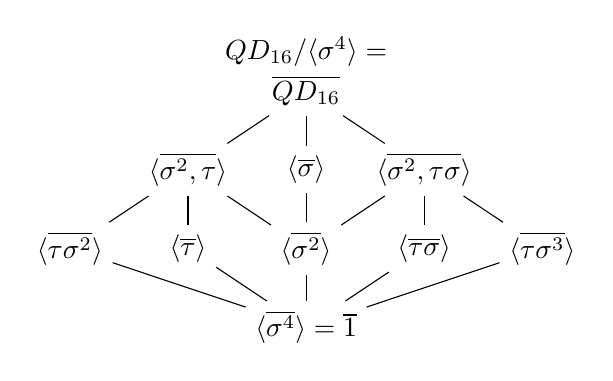
\begin{tikzpicture}
            \node at (0, 0)          (1)  {$\langle \overline{\sigma^4} \rangle = \overline{1}$};

            \node at (-3, 1)      (ts2)  {$\langle \overline{\tau \sigma^2} \rangle$};
            \node at (-1.5, 1)      (t) {$\langle \overline{\tau} \rangle$};
            \node at (0, 1)      (s2) {$\langle \overline{\sigma^2} \rangle$};
            \node at (1.5, 1)      (ts) {$\langle \overline{\tau \sigma} \rangle$};
            \node at (3, 1)      (ts3) {$\langle \overline{\tau \sigma^3} \rangle$};

            \node at (-1.5, 2)      (s2_t) {$\langle \overline{\sigma^2, \tau} \rangle$};
            \node at (0, 2)      (s) {$\langle \overline{\sigma} \rangle$};
            \node at (1.5, 2)      (s2_ts) {$\langle \overline{\sigma^2, \tau \sigma} \rangle$};
            \node at (0, 3.5)       ()  {$QD_{16}/\langle \sigma^4 \rangle =$};
            \node at (0, 3)       (QD16)  {$\overline{QD_{16}}$};
            
            \draw (1) -- (ts2);
            \draw (1) -- (t);
            \draw (1) -- (s2);
            \draw (1) -- (ts);
            \draw (1) -- (ts3);

            \draw(ts2) -- (s2_t);
            \draw(t) -- (s2_t);
            \draw(s2) -- (s2_t);
            \draw(s2) -- (s);
            \draw(s2) -- (s2_ts);
            \draw(ts) -- (s2_ts);
            \draw(ts3) -- (s2_ts);

            \draw(s2_t) -- (QD16);
            \draw(s) -- (QD16);
            \draw(s2_ts) -- (QD16);
        \end{tikzpicture}
    \end{center}

    Next, consider the generators and relations for $\overline{QD_{16}}$:
    \begin{equation*}
        \overline{QD_{16}} = \langle \overline{\sigma}, \overline{\tau} \mid \overline{\sigma}^4 = \overline{\tau}^2 = \overline{1}, \overline{\sigma \tau} = \overline{\tau \sigma^3} = \overline{\tau} \cdot \overline{\sigma}^{-1} \rangle.
    \end{equation*}
    The right-most equation among the relations: $\overline{\tau \sigma^3} = \overline{\tau} \cdot \overline{\sigma}^{-1}$ shows that the generators and relations of this quotient group are identical to those of $D_8$, mapping $s \in D_8$ to $\overline{\tau} \in \overline{QD_{16}}$ and $r \in D_8$ to $\overline{\sigma} \in \overline{QD_{16}}$. Thus we have $QD_{16}/\langle \sigma^4 \rangle \cong D_8$.
\end{proof}

\section*{6. (10/28/23)}

Let $M = \langle v, u \rangle$ be the modular group of order 16 described in Exercise 14 of Section 2.5. Prove that $\langle v^4 \rangle$ is normal in $M$ and use the Lattice Isomorphism Theorem to draw the lattice of subgroups of $M/\langle v^4 \rangle$. Which group of order 8 has the same lattice as this quotient? Use generators and relations for $M/\langle v^4 \rangle$ to decide the isomorphism type of this group.

\begin{proof}[Solution]
    Recall that the modular group of order 16 is defined as:
    \begin{equation*}
        M = \langle v, u \mid u^2 = v^8 = 1, vu = uv^5 \rangle.
    \end{equation*}
    As above, to show that $\langle v^4 \rangle$ is normal in $M$, it suffices to show that the conjugate $uv^4u^{-1}$ lies in $\langle v^4 \rangle$:
    \begin{equation*}
        uv^4u^{-1} = uv^4u = uuv^{20} = v^{4} \in \langle v^4 \rangle,
    \end{equation*}
    so $\langle v^4 \rangle \unlhd M$.

    From the Lattice Isomorphism Theorem, the lattice of subgroups of $M/\langle v^4 \rangle$ corresponds to the lattice of subgroups of $M$ containing $\langle v^4 \rangle$:

    \begin{center}
        \begin{tikzpicture}
            \node at (0, 0)          (1)  {$\langle \overline{v^4} \rangle = \overline{1}$};

            \node at (-3, 1)      (uv2)  {$\langle \overline{u v^2} \rangle$};
            \node at (-1.5, 1)      (u) {$\langle \overline{u} \rangle$};
            \node at (0, 1)      (v2) {$\langle \overline{v^2} \rangle$};
            \node at (1.5, 1)      (uv) {$\langle \overline{u v} \rangle$};
            \node at (3, 1)      (uv3) {$\langle \overline{u v^3} \rangle$};

            \node at (-1.5, 2)      (v2_u) {$\langle \overline{v^2, u} \rangle$};
            \node at (0, 2)      (v) {$\langle \overline{v} \rangle$};
            \node at (1.5, 2)      (v2_uv) {$\langle \overline{v^2, u v} \rangle$};
            \node at (0, 3.5)       ()  {$M/\langle v^4 \rangle =$};
            \node at (0, 3)       (M)  {$\overline{M}$};
            
            \draw (1) -- (uv2);
            \draw (1) -- (u);
            \draw (1) -- (v2);
            \draw (1) -- (uv);
            \draw (1) -- (uv3);

            \draw(ts2) -- (v2_u);
            \draw(t) -- (v2_u);
            \draw(v2) -- (v2_u);
            \draw(v2) -- (v);
            \draw(v2) -- (v2_uv);
            \draw(ts) -- (v2_uv);
            \draw(uv3) -- (v2_uv);

            \draw(s2_t) -- (M);
            \draw(v) -- (M);
            \draw(v2_uv) -- (M);
        \end{tikzpicture}
    \end{center}


    Next, consider the generators and relations for $M/\langle v^4 \rangle$:
    \begin{equation*}
        M/\langle v^4 \rangle = \langle \overline{v}, \overline{u} \mid \overline{v}^4 = \overline{u}^2 = \overline{1}, \overline{v u} = \overline{u v^5} = \overline{uv} \rangle.
    \end{equation*}

    The right-most equation shows that this is an abelian group. Consider the presentation for $Z_2 \times Z_4$ given by $\langle x, y \mid x^2 = y^4 = 1, xy = yx \rangle$. Mapping $\overline{u} \in M/\langle v^4 \rangle$ to $x \in Z_2 \times Z_4$ and $\overline{v} \in M/\langle v^4 \rangle$ to $y \in Z_2 \times Z_4$, we obtain an isomorphism. Therefore $M/\langle v^4 \rangle \cong Z_2 \times Z_4$.
\end{proof}

\section*{7. (10/28/23)}

Let $M$ and $N$ be normal subgroups of $G$ such that $G = MN$. Prove that $G/(M \cap N) \cong (G/M) \times (G/N)$.

\begin{proof}
    Define a map $\varphi: G/(M \cap N) \rightarrow (G/M) \times (G/N)$ by $\varphi(\overline{g}) = (gM, gN)$. We see that $\varphi$ is a homomorphism:
    \begin{multline*}
        \varphi(\overline{g} \cdot \overline{h}) = \varphi(\overline{gh}) = ((gh)M, (gh)N) = (gM \cdot hM, gN \cdot hN) \\ = (gM, gN)(hM, hN) = \varphi(\overline{g})\varphi(\overline{h}).
    \end{multline*}

    It is also injective. Let $\varphi(\overline{g}) = \varphi(\overline{h})$, so $(gM, gN) = (hM, hN)$, which implies that $gM = hM$ and $gN = hN$. Now let $x \in M \cap N$, so $x \in M$ and $x \in N$. Then $gx \in hM$ (because $gM = hM$) and $gx \in hN$ (because $gN = hN$), so $gx \in hM \cap hN = h(M \cap N)$. The same logic shows that $hx \in g(M \cap N)$, and it follows that $g(M \cap N) = h(M \cap N) \Rightarrow \overline{g} = \overline{h}$, which proves that $\varphi$ is injective.

    Finally, $\varphi$ is surjective. Let $(gM, hN)$ be an element of $(G/M) \times (G/N)$. Since $G = MN = \{ mn \mid m \in M, n \in N \}$, we can write:
    \begin{multline*}
        (gM, hN) = \underbrace{((m_1 n_1)M, (m_2 n_2)N)}_{\text{for some $m_1, m_2 \in M, n_1, n_2 \in N$}} \\ = (n_1 M, m_2 N) = ((m_2 n_1) M, (m_2 n_1) N) = \varphi(\overline{m_2 n_1}).
    \end{multline*}
    Thus $\varphi$ is an isomorphism, and so $G/(M \cap N) \cong (G/M) \times (G/N)$.
\end{proof}

\section*{8. (10/29/23)}

Let $p$ be a prime and let $G$ be the group of $p$-power roots of 1 in $\mathbb{C}$ (cf. Exercise 18, Section 2.4). Prove that the map $z \mapsto z^p$ is a surjective homomorphism. Deduce that $G$ is isomorphic to a proper quotient of itself.

\begin{proof}
    Recall that $G = \{ z \in \mathbb{C} \mid z^{p^n} = 1 \text{ for some } n \in \mathbb{Z}^+ \}$. Define a map $\varphi: G \rightarrow G$ by $\varphi(z) = z^p$ for all $z \in G$. Since $\varphi(z_1 z_2) = (z_1 z_2)^p = z_1^p z_2^p = \varphi(z_1) \varphi(z_2)$, it is a homomorphism.

    To show that $\varphi$ is surjective, let $y \in G$. In particular, let $y = e^{\frac{2 \pi i}{p^n}}$ for some $n \in \mathbb{Z}^+$. Let $z = y^{1/p}$. Then $\varphi(z) = z^p = (y^{1/p})^p = y$. And, because $z = y^{1/p} = e^{\frac{2 \pi i}{p^n} \cdot \frac{1}{p}} = e^{\frac{2 \pi i}{p^{n + 1}}}$, we have $z^{p^{n + 1}} = 1$, so $z \in G$. Therefore $\varphi$ is also surjective.

    By the 1st Isomorphism Theorem, $\ker \varphi \unlhd G$ and $G / \ker \varphi \cong \varphi(G)$. Now the kernel of $\varphi$ is the set of those $z \in G$ such that $z^p = 1$, that is, $\langle e^{\frac{2 \pi i}{p}} \rangle$. So $G / \ker \varphi$ is a proper quotient of $G$. Since $\varphi$ is surjective, $\varphi(G) = G$, and therefore $G$ is isomorphic to a proper quotient of itself.
\end{proof}

\section*{9. (10/29/23)}

Let $p$ be a prime and let $G$ be a group of order $p^a m$, where $p$ does not divide $m$. Assume $P$ is a subgroup of $G$ of order $p^a$ and $N$ is a normal subgroup of $G$ of order $p^b n$, where $p$ does not divide $n$. Prove that $|P \cap N| = p^b$ and $|PN / N| = p^{a - b}$. (The subgroup $P$ of $G$ is called a \emph{Sylow $p$-subgroup} of $G$. This exercise shows that the intersection of any Sylow $p$-subgroup of $G$ with a normal subgroup $N$ is a Sylow $p$-subgroup of $N$.)

\begin{proof}
    Since $P \cap N \leq P$ and $P \cap N \leq N$, the order of $P \cap N$ must divide $|P| = p^a$ and $|N| = p^b n$. And since the order of $N$ divides the order of $G$, we must have $b \leq a$. Therefore $|P \cap N| = p^c$ for some $c \leq b \leq a$.

    Suppose that $c < a$. From the Diamond Isomorphism Theorem, $P \cap N \unlhd P$, so we have:
    \begin{equation*}
        |P : P \cap N| = |P / P \cap N| = \frac{|P|}{|P \cap N|} = \frac{p^a}{p^c} = p^{a - c}.
    \end{equation*}
    The Diamond Isomorphism Theorem also states that $PN / N \cong P / P \cap N$, which implies that $\frac{|PN|}{|N|} = p^{a - c}$. We know that the order of $N$ is $p^b n$, and so $|PN| = p^{a - c} p^b n = p^{a + b - c} n$. Now note that $a + b - c > a$, which contradicts the order of $N$ dividing the order of $G$. Therefore we must have $c = b$, and so $|P \cap N| = p^b$. Again, because $PN / N \cong P / P \cap N$, we obtain $|PN / N| = p^{a - b}$.
\end{proof}

\section*{10. (11/2/23)}

Generalize the preceding exercise as follows. A subgroup $H$ of a finite group $G$ is called a \emph{Hall subgroup} of $G$ if its index is relatively prime to its order: $(|G:H|, |H|) = 1$. Prove that if $H$ is a Hall subgroup of $G$ and $N \unlhd G$, then $H \cap N$ is a Hall subgroup of $N$ and $HN/N$ is a Hall subgroup of $G/N$.

\begin{proof}
    We wish to first show that $H \cap N$ is a Hall subgroup of $N$, that is, that $|H \cap N|$ and $|N : H \cap N|$ are relatively prime.
    
    Toward contradiction, let $x > 1$ divide both $|H \cap N|$ and $|N : H \cap N|$. Since $H \cap N \leq H$, $x$ also divides $|H|$. By Proposition 13,
    \begin{equation*}
        |HN| = \frac{|H||N|}{|H \cap N|} = |H| \frac{|N|}{|H \cap N|} = |H||N : H \cap N|.
    \end{equation*}
    By Corollary 15, $HN$ is a subgroup of $G$, so $|HN|$ divides $|G| = |H|\frac{|G|}{|H|}$. Since $|H|$ and $|G : H| = \frac{|G|}{|H|}$ are relatively prime, $|N : H \cap N|$ divides $\frac{|G|}{|H|}$. But if $x$ divides $|H|$, it does not divide $\frac{|G|}{|H|}$, and therefore also does not divide $|N : H \cap N|$, a contradiction. So we must have $x = 1$, which implies that $|H \cap N|$ and then $|N : H \cap N|$ are relatively prime, and $H \cap N$ is a Hall subgroup of $N$.

    Next, consider $HN/N \leq G/N$. We wish to show that $HN/N$ is a Hall subgroup of $G/N$, that is, that $|HN/N|$ and $|G/N : HN / N|$ are relatively prime. Again suppose that $x > 1$ divides both $|HN/N|$ and $|G/N : HN / N|$. From the Diamond Isomorphism Theorem, $HN/N \cong H/H \cap N$, so $x$ divides $|H/H \cap N| = \frac{|H|}{|H \cap N|}$, and therefore $x$ divides the order of $H$. And, from the Third Isomorphism Theorem, $(G/N)/(HN/N) \cong G/HN$, so:
    \begin{align*}
        |G/N : HN / N| = |G:HN| = \frac{|G|}{|HN|} &= |G|\frac{|H \cap N|}{|H||N|} \\ &= \frac{|G|}{|H|} \cdot \frac{|H \cap N|}{|N|} = \frac{|G|}{|H|} \cdot \frac{1}{|N:H \cap N|}.
    \end{align*}
    By assumption, $x$ divides this, and so it also divides $\frac{|G|}{|H|} = |G:H|$. However, because $H$ is a Hall subgroup of $G$, this is a contradiction if $x > 1$. Therefore we must have $x = 1$, so $HN/N$ is a Hall subgroup of $G/N$.
\end{proof}

\end{document}